% -----------------------------*- LaTeX -*------------------------------
\documentclass[12pt]{report}
\usepackage{scribe_hgen486}
\usepackage{tikz}
\usetikzlibrary{bayesnet}
\usepackage{hyperref}
\begin{document}

\lecturer{John Novembre}		% optional
\scribe{Matt Bonakdarpour}		% required
\lecturenumber{2}			% required, must be a number
\lecturedate{January 7}		        % required, omit year

\maketitle

\framebox[.95\textwidth]{\parbox{.93\textwidth}{ {{\bf Note:}} These
lecture notes are still rough, and have only have been mildly
proofread.  }}
\vspace*{.1in}
\setlength{\parindent}{0cm}



% ----------------------------------------------------------------------
\section{Graphical Models: Introduction}
Quite often, we are confronted with the task of understanding a complex system
with many dependent components. In this context, probability theory
gives us a framework to reason about a collection of possible outcomes
and their associated likelihoods. For example, if we are trying to
diagnose a patient, there are many potential diseases this patient
could have. Also, associated with each patient, we may have hundreds
of data points related to their symptoms, personal traits, and
diagnostic tests. Each of these characteristics could be thought of as
a random variable. Our goal is to reason about this patient given the
values of one or more of these random variables. In the framework of
probabilistic reasoning, we need to construct a joint distribution
over the space of possible assignments to this set of random
variables. 

If we have five realizations of \emph{binary} random variables for a patient, we must specify a joint
distribution over $2^5$ possible values -- a potentially daunting task! Graphical models provide a
framework to compactly encode a joint distribution in high
dimensions. They also provide other benefits, including but not
limited to:
\begin{itemize}
\item A tool for visualizing the structure of a probabilistic model
\item Provides insights, such as conditional independence properties, by inspection of the graph
\item Complex computations can be expressed as operations on the graph
\end{itemize}

In this lecture, we will consider directed graphical models, sometimes
known as Bayesian networks. 

\subsection{Joint probabilities and independence}
Using the definition of conditional probability, we have that the
joint distribution between $X_i$ and $X_j$ is:
\begin{align*}
p(X_i,X_j) = P(X_i | X_j)P(X_j)
\end{align*}

In general, if we have any $n$ random variables $X_1,\ldots,X_n$, we can
use the \emph{chain rule} to factor the joint distribution as follows:
\begin{align*}
p(X_1,\ldots,X_n) = p(X_1)p(X_2|X_1)p(X_3|X_1,X_2)\cdots
p(X_n|X_1,\ldots ,X_{n-1})
\end{align*}

Recall that $X_i$ is independent of $X_j$ if knowledge of $X_j$ does
not change our knowledge of $X_i$. That is, $p(X_i | X_j) =
p(X_i)$. Plugging this in to the expression for the joint distribution
above, we have that $X_i$ is independent of $X_j$ if and only if
$p(X_i,X_j)=p(X_i)p(X_j)$.

We say that $X_i$ is \emph{conditionally independent} of $X_j$ given
$X_k$ if
\begin{align*}
p(X_i,X_j|X_k) = p(X_i|X_k)p(X_j|X_k)
\end{align*}
which means
\begin{align*}
p(X_i,X_j,X_k) = p(X_i|X_k)p(X_j|X_k)p(X_k)
\end{align*}

Notice how the joint distribution factorizes nicely when we have
conditional independence. Idea: when faced with a large number of
features, use our prior knowledge of independence to simplify the
joint distribution. 

\subsection{Some basics}
A directed graph is a set of vertices (or nodes) along with a set of
directed edges (or arrows) between nodes. Here is a simple graph with
two vertices and one directed edge:

\begin{center}
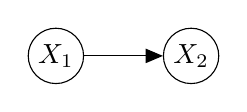
\begin{tikzpicture}

  % Define nodes
  \node[latent]                             (x1) {$X_1$};
  \node[latent,right=of x1]                 (x2) {$X_2$};

  \edge {x1} {x2} ; %
\end{tikzpicture}
\end{center}

Here, each vertex represents a random variable. When a specific random
variable in the graph is observed, we shade that particular
vertex. For example, this is what the graph above would look like if
we observed $X_1$, but $X_2$ was still latent:

\begin{center}
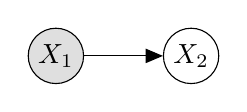
\begin{tikzpicture}

  % Define nodes
  \node[obs]                             (x1) {$X_1$};
  \node[latent,right=of x1]                 (x2) {$X_2$};

  \edge {x1} {x2} ; %
\end{tikzpicture}
\end{center}

A directed graphical model encodes conditional independence in the
following way. A specific random variable (or vertex) is conditionally
independent of all other nodes, given its parents (i.e. all nodes that
points to it). For example, in the following graph $X_1$ is
independent of $X_3$ given $X_2$:

\begin{center}
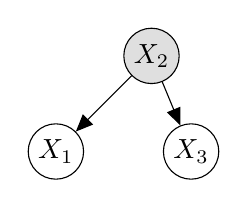
\begin{tikzpicture}

  % Define nodes
  \node[obs]                                (x2) {$X_2$};
  \node[latent,below left=of x2]                 (x1) {$X_1$};
  \node[latent,below right=of x2, right=of x1]                 (x3) {$X_3$};

  \edge {x2} {x1} ; %
  \edge {x2} {x3} ; %
\end{tikzpicture}
\end{center}
The general form for the joint distribution for a directed graphical
model is therefore:
\begin{align}
p(X_1,\ldots,X_n) = \prod_{i=1}^n p(X_i |\text{pa}_i) \label{eq:gm_prob}
\end{align}
where $\text{pa}_i$ denotes the parents of $X_i$.
\subsection{A motivating example}
Assume we have 3 possible genotypes $\{$AA,Aa,aa$\}$. To each person, we will assign a
random variable $X_i$ according to their genotype:
\begin{center}
\begin{tabular}{l|l }
  Genotype & $X_i$ \\
  \hline
  AA & 0 \\
  Aa & 1 \\
  aa & 2 
\end{tabular}
\end{center}
Let's also assume that the genotype of each person is binomially
distributed, so that:
\begin{align*}
X_i|p &\sim \text{Bin}(2,p) \\
p(X_i=2|p) &= p^2 \\
p(X_i=1|p) &= 2p(1-p) \\
p(X_i=0|p) &= (1-p)^2
\end{align*}
In this context, we represent inheritance in a 3-generation
pedigree with the following graphical model. In what follows, we're
assuming $X_8 = p$.

\begin{center}
\begin{tikzpicture}

  % Define nodes
  \node[obs]                               (x8) {$X_8$};
  \node[latent,below left=of x8, right of=x1]                 (x2)
  {$X_2$};
  \node[latent,below left =of x8, left=of x2]                 (x1) {$X_1$};
  \node[latent,below right=of x8, right=of x2]                 (x3) {$X_3$};
  \node[latent,below right=of x8, right=of x3]                 (x4)
  {$X_4$};

  \node[latent,below right=of x1, below left=of x2]                 (x5) {$X_5$};
  \node[latent,below right=of x3, below left=of x4]                 (x6)
  {$X_6$};

  \node[latent,below right=of x5, below left=of x6]                 (x7) {$X_7$};


  % Connect the nodes
  \edge {x8} {x1,x2,x3,x4} ; %
  \edge {x1,x2} {x5} ; %
  \edge {x3,x4} {x6} ; %
  \edge {x5,x6} {x7} ; %
\end{tikzpicture}
\end{center}

Assume $X_8$ is observed and that we are interested in
$p(X_5|X_1,X_2)$. We could represent this conditional probability as a
table, enumerating all possibly quantities that $X_1,X_2$ and $X_5$
take. In general, we can represent $P(X_i | X_j,X_k)$ where $X_i$ is
the child of $X_j$ and $X_k$ using the basic laws of Mendelism:
\begin{center}
\begin{tabular}{|c c|c c c|}
\hline
Father & Mother & \multicolumn{3}{c|}{Child ($X_i$)} \\
$X_j$ & $X_k$ &           0 &           1 &           2 \\
\hline
0     & 0     &           1 &           0 &           0 \\
0     & 1     & $\frac{1}{2}$ & $\frac{1}{2}$ &           0 \\
0     & 2     &           0 &           1 &           0 \\
1     & 0     & $\frac{1}{2}$ & $\frac{1}{2}$ &           0 \\
1     & 1     & $\frac{1}{4}$ & $\frac{1}{2}$ & $\frac{1}{4}$ \\
1     & 2     &           0 & $\frac{1}{2}$ & $\frac{1}{2}$ \\
2     & 0     &           0 &           1 &           0 \\
2     & 1     &           0 & $\frac{1}{2}$ & $\frac{1}{2}$ \\
2     & 2     &           0 &           0 &           1 \\
\hline
\end{tabular}
\end{center}

From the graphical model above, and using equation~\ref{eq:gm_prob},
we can factorize the joint distribution in the following way, in which
the values of the table above can be used to compute the joint distribution:
\begin{align*}
p(X_1,\ldots,X_8) = p(X_1|X_8)p(X_2|X_8)p(X_3|X_8)p(X_4|X_8)\times \\p(X_5|X_1,X_2)p(X_6|X_3,X_4)p(X_7|X_5,X_6)p(X_8)
\end{align*}



\subsection{Some classes of 3-node graphs}

With the linear chain graph, we have that $X_1 \perp X_3 | X_2$:

\begin{center}
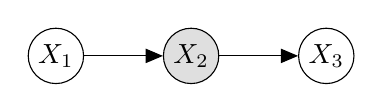
\begin{tikzpicture}

  % Define nodes
  \node[obs]                                (x2) {$X_2$};
  \node[latent,left=of x2]                 (x1) {$X_1$};
  \node[latent,right=of x2]                 (x3) {$X_3$};

  \edge {x1} {x2} ; %
  \edge {x2} {x3} ; %
\end{tikzpicture}
\end{center}

As we saw in a previous section, in this multiple offspring graph, we
have that $X_1 \perp~ X_3 | X_2$:

\begin{center}
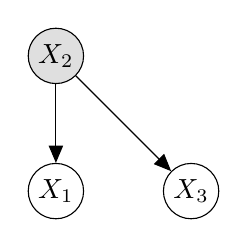
\begin{tikzpicture}

  % Define nodes
  \node[obs]                                (x2) {$X_2$};
  \node[latent,below=of x2]                 (x1) {$X_1$};
  \node[latent,right=of x1]                 (x3) {$X_3$};

  \edge {x2} {x1} ; %
  \edge {x2} {x3} ; %
\end{tikzpicture}
\end{center}

The v-structure graph has the following structure:
\begin{center}
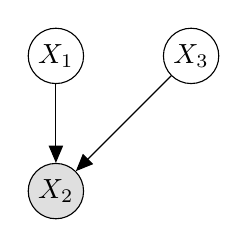
\begin{tikzpicture}

  % Define nodes
  \node[obs]                                (x2) {$X_2$};
  \node[latent,above=of x2]                 (x1) {$X_1$};
  \node[latent,right=of x1]                 (x3) {$X_3$};

  \edge {x1} {x2} ; %
  \edge {x3} {x2} ; %
\end{tikzpicture}
\end{center}
In this case, it is \emph{not true} that $X_1 \perp X_3 | X_2$. For example, assume
$X_2$ was the event that your house alarm was going off, $X_1$ was the
event that there was an earthquake, and $X_3$ was the event that there
was a burglar in your house. Assuming your alarm was going off, the
additional information about whether a burglar was in your house would
affect your knowledge of whether or not an earthquake was
happening.

\subsection{D-separation}
Take any undirected path (ignoring arrows) in the graph $G$. This path
is called an \emph{active trail} for observed variables $O \subset
\{X_1,\ldots,X_n\}$, if for every consecutive triple of variables
$X,Y,Z$ on the path:
\begin{itemize}
\item $X \rightarrow Y \rightarrow Z$ and $Y\not\in O$
\item $X \leftarrow Y \leftarrow Z$ and $Y\not\in O$
\item $X \leftarrow Y \rightarrow Z$ and $Y\not\in O$
\item $X\rightarrow Y \leftarrow Z$ and $Y$ or any of $Y$'s
  descendants are in $O$
\end{itemize}

Any two variables $X_i$ and $X_j$ for which there does not exist an
active trail for observations $O$ are called \emph{d-separated} by
$O$, written d-sep($X_i;X_j|O$). Two sets of vertices $A$ and $B$ are
d-separated by $O$ if d-sep($X,Y|O$) for all $X\in A$ and $Y\in B$. 

The key result is the following: if $X$ and $Y$ are d-separated by a
set $O$, then $X \perp Y | O$. In words, $X$ is conditionally
independent of $Y$ given $O$ if there does not exist any active trail
between $X$ and $Y$ for observations $O$. Intuition: active trails allow the
dependencies to flow. 

\subsection{Elimination Algorithm}
Assume we have a graph $G$, and we take two disjoint subsets of
nodes $X_E$ and $X_Q$. Our goal is to calculate $p(X_Q|X_E)$. In this
section, we will focus on the case when $X_Q$ is one node called the
\emph{query node}, and the set of nodes $X_E$ are called
\emph{evidence nodes}.

Assume we have the following graph:
\begin{center}
\begin{tikzpicture}

  % Define nodes
  \node[latent]                              (x1) {$X_1$};
  \node[latent, above right=of x1]              (x2) {$X_2$};
  \node[latent, below right=of x3, below=of x2]                              (x3) {$X_3$};
  \node[latent, above right=of x2]                              (x4) {$X_4$};
  \node[latent, right=of x3]                              (x5) {$X_5$};
  \node[obs, above right=of x5, below=of x4, right=of x5]                              (x6) {$X_6$};


  \edge {x1} {x2} ; %
  \edge {x1} {x3} ; %
  \edge {x2} {x4} ; %
  \edge {x2} {x6} ; %
  \edge {x3} {x5} ; %
  \edge {x5} {x6} ; %
\end{tikzpicture}
\end{center}
Let our evidence set be $\{X_6\}$ and our query set be $\{X_1\}$. We
want to compute:
\begin{align*}
p(X_1|X_6) = \frac{p(X_1,X_6)}{p(X_6)} = \frac{p(X_1,X_6)}{\sum_{x_1}p(X_1=x_1,X_6)}
\end{align*}
The elimination algorithm provides an effective computational method
for making these calculations. 

From the expression above, it seems that to compute the conditional distribution, we just need to be able to
compute the joint distribution $p(X_1,X_6)$. We could start off by
marginalizing the full joint distribution for all variables:
\begin{align*}
p(X_1,X_6) = \sum_{x_2}\sum_{x_3}\sum_{x_4}\sum_{x_5}p(X_1,X_2,\ldots,X_6)
\end{align*}
In this case,if every $X_i$ can take on one of $k$ values, this expression would
have $k^4$ terms. However, using the conditional independence
relations from the graph, we get:
\begin{align*}
p(X_1,X_6) &=
\sum_{x_2}\sum_{x_3}\sum_{x_4}\sum_{x_5}p(X_1)p(X_2|X_1)p(X_3|X_1)p(X_4|X_2)p(X_5|X_3)p(X_6|X_2,X_5)
\\
&=p(X_1)p\sum_{x_2}(X_2|X_1)\sum_{x_3}p(X_3|X_1)\sum_{x_4}p(X_4|X_2)\sum_{x_5}p(X_5|X_3)p(X_6|X_2,X_5)
\end{align*}
We can further simplify this summation by introducing the following
notation. Let $m_i(x_{S_i})$ denote the expression that arises when
performing the sum $\sum_{x_i}$ where $x_{S_i}$ are the variables,
other than $x_i$ that appear in the summand. Employing this notation,
we get:
\begin{align*}
p(X_1,X_6) &=
p(X_1)p\sum_{x_2}(X_2|X_1)\sum_{x_3}p(X_3|X_1)\underbrace{\sum_{x_4}p(X_4|X_2)}_{m_4(x_2)}\underbrace{\sum_{x_5}p(X_5|X_3)p(X_6|X_2,X_5)}_{m_5(x_2,x_3)}
\\
&=
p(X_1)p\sum_{x_2}(X_2|X_1)m_4(x_2)\underbrace{\sum_{x_3}p(X_3|X_1)m_5(x_2,x_3)}_{m_3(x_1,x_2)}
= p(X_1)p\sum_{x_2}(X_2|X_1)m_4(x_2)m_3(x_1,x_2) \\
&= p(x_1)m_2(x_1) \\
\end{align*}
Using this result, we get the desired conditional probability:
\begin{align*}
\Rightarrow p(X_1|X_6) &= \frac{p(x_1)m_2(x_1)}{\sum_{x_1}p(x_1)m_2(x_1)}
\end{align*}
This exercise gives rise to a general algorithm for computing marginal
probabilities. To see the details of this algorithm, refer to the
handout given in class entitled \emph{The Elimination Algorithm}.

In statistical genetics, Felsenstein's tree-pruning algorithm (1981, JME) computes
the likelihood of an evolutionary tree from nucleic acid sequence
data. This pruning algorithm was an early instance of the elimination
algorithm. As a simplified illustration, we can represent a phylogeny
as a tree in which the leaves correspond to the \emph{observed} values
of a site across different species. The non-leaves are values of the site
for the ancestors. Each edge of the tree can represent the
\emph{evolutionary distance} to be estimated which can be encoded as the
conditional probability of a state given its ancestral state. Using
Felsenstein's pruning algorithm, we can obtain the joint probability
across all sites. This can be used in conjunction with the EM
algorithm to find the maximum likelihood tree. 

\\
Relevant online course notes:
\begin{itemize}
\item \url{http://www.inf.ed.ac.uk/teaching/courses/pmr/slides/elim-2x2.pdf}
\item \url{https://www.cs.cmu.edu/~aarti/Class/10701/readings/graphical_model\_Jordan.pdf}
\item \url{http://www.cs.columbia.edu/~blei/fogm/2015F/notes/inference.pdf}
\item \url{http://www.cs.berkeley.edu/~jordan/courses/281A-fall04/}
\end{itemize}
For drawing graphical models
\begin{itemize}
\item \url{https://github.com/jluttine/tikz-bayesnet}
\end{itemize}

\end{document}

